%\documentclass[acmsmall,screen,review]{acmart}
%\documentclass[acmconf,screen,review]{acmart}
\documentclass[screen,review]{acmart}
\usepackage{todonotes}
\usepackage{comment}
%%
%% \BibTeX command to typeset BibTeX logo in the docs
\AtBeginDocument{%
  \providecommand\BibTeX{{%
    \normalfont B\kern-0.5em{\scshape i\kern-0.25em b}\kern-0.8em\TeX}}}

%% Rights management information.  This information is sent to you
%% when you complete the rights form.  These commands have SAMPLE
%% values in them; it is your responsibility as an author to replace
%% the commands and values with those provided to you when you
%% complete the rights form.
\setcopyright{acmcopyright}
\copyrightyear{2021}
\acmYear{2021}
\acmDOI{}

%% These commands are for a PROCEEDINGS abstract or paper.
\acmConference[JCDL '21]{JCDL '21: Joint Conference on
  Digital Libraries, September 27--30, 2021, Urbana--Champaign, Illinois, USA}
%\acmBooktitle{Woodstock '18: ACM Symposium on Neural Gaze Detection,
  %June 03--05, 2018, Woodstock, NY}
%\acmPrice{15.00}
%\acmISBN{978-1-4503-XXXX-X/18/06}


%%
%% Submission ID.
%% Use this when submitting an article to a sponsored event. You'll
%% receive a unique submission ID from the organizers
%% of the event, and this ID should be used as the parameter to this command.
%%\acmSubmissionID{123-A56-BU3}

%%
%% The majority of ACM publications use numbered citations and
%% references.  The command \citestyle{authoryear} switches to the
%% "author year" style.
%%
%% If you are preparing content for an event
%% sponsored by ACM SIGGRAPH, you must use the "author year" style of
%% citations and references.
%% Uncommenting
%% the next command will enable that style.
%%\citestyle{acmauthoryear}

%%
%% end of the preamble, start of the body of the document source.
\begin{document}

%%
%% The "title" command has an optional parameter,
%% allowing the author to define a "short title" to be used in page headers.
\title{Automated Metadata Generation for Fish Specimen Image Collections}

%%
%% The "author" command and its associated commands are used to define
%% the authors and their affiliations.
%% Of note is the shared affiliation of the first two authors, and the
%% "authornote" and "authornotemark" commands
%% used to denote shared contribution to the research.
\author{Joel Pepper}
\email{jcp353@drexel.edu}
\orcid{0002-1601-8729}
\author{Jane Greenberg}
\author{David Breen}
\orcid{0002-1376-5008}
\affiliation{%
  \institution{Drexel University}
  \streetaddress{3675 Market St}
  \city{Philadelphia}
  \state{Pennsylvania}
  \country{USA}
  \postcode{19104}
}

%%
%% By default, the full list of authors will be used in the page
%% headers. Often, this list is too long, and will overlap
%% other information printed in the page headers. This command allows
%% the author to define a more concise list
%% of authors' names for this purpose.
\renewcommand{\shortauthors}{Pepper, Greenberg and Breen}

%%
%% The abstract is a short summary of the work to be presented in the
%% article.
\begin{abstract}
  A clear\todo{test} and well-documented \LaTeX\ document is presented as an
  article formatted for publication by ACM in a conference proceedings
  or journal publication. Based on the ``acmart'' document class, this
  article presents and explains many of the common variations, as well
  as many of the formatting elements an author may use in the
  preparation of the documentation of their work.
\end{abstract}

%%
%% The code below is generated by the tool at http://dl.acm.org/ccs.cfm.
%% Please copy and paste the code instead of the example below.
%%
\begin{CCSXML}
<ccs2012>
   <concept>
       <concept_id>10002951.10002952.10003219.10003215</concept_id>
       <concept_desc>Information systems~Extraction, transformation and loading</concept_desc>
       <concept_significance>500</concept_significance>
       </concept>
 </ccs2012>
\end{CCSXML}

\ccsdesc[500]{Information systems~Extraction, transformation and loading}

%%
%% Keywords. The author(s) should pick words that accurately describe
%% the work being presented. Separate the keywords with commas.
\keywords{bioinformatics, metadata}

%% A "teaser" image appears between the author and affiliation
%% information and the body of the document, and typically spans the
%% page.
\begin{teaserfigure}
  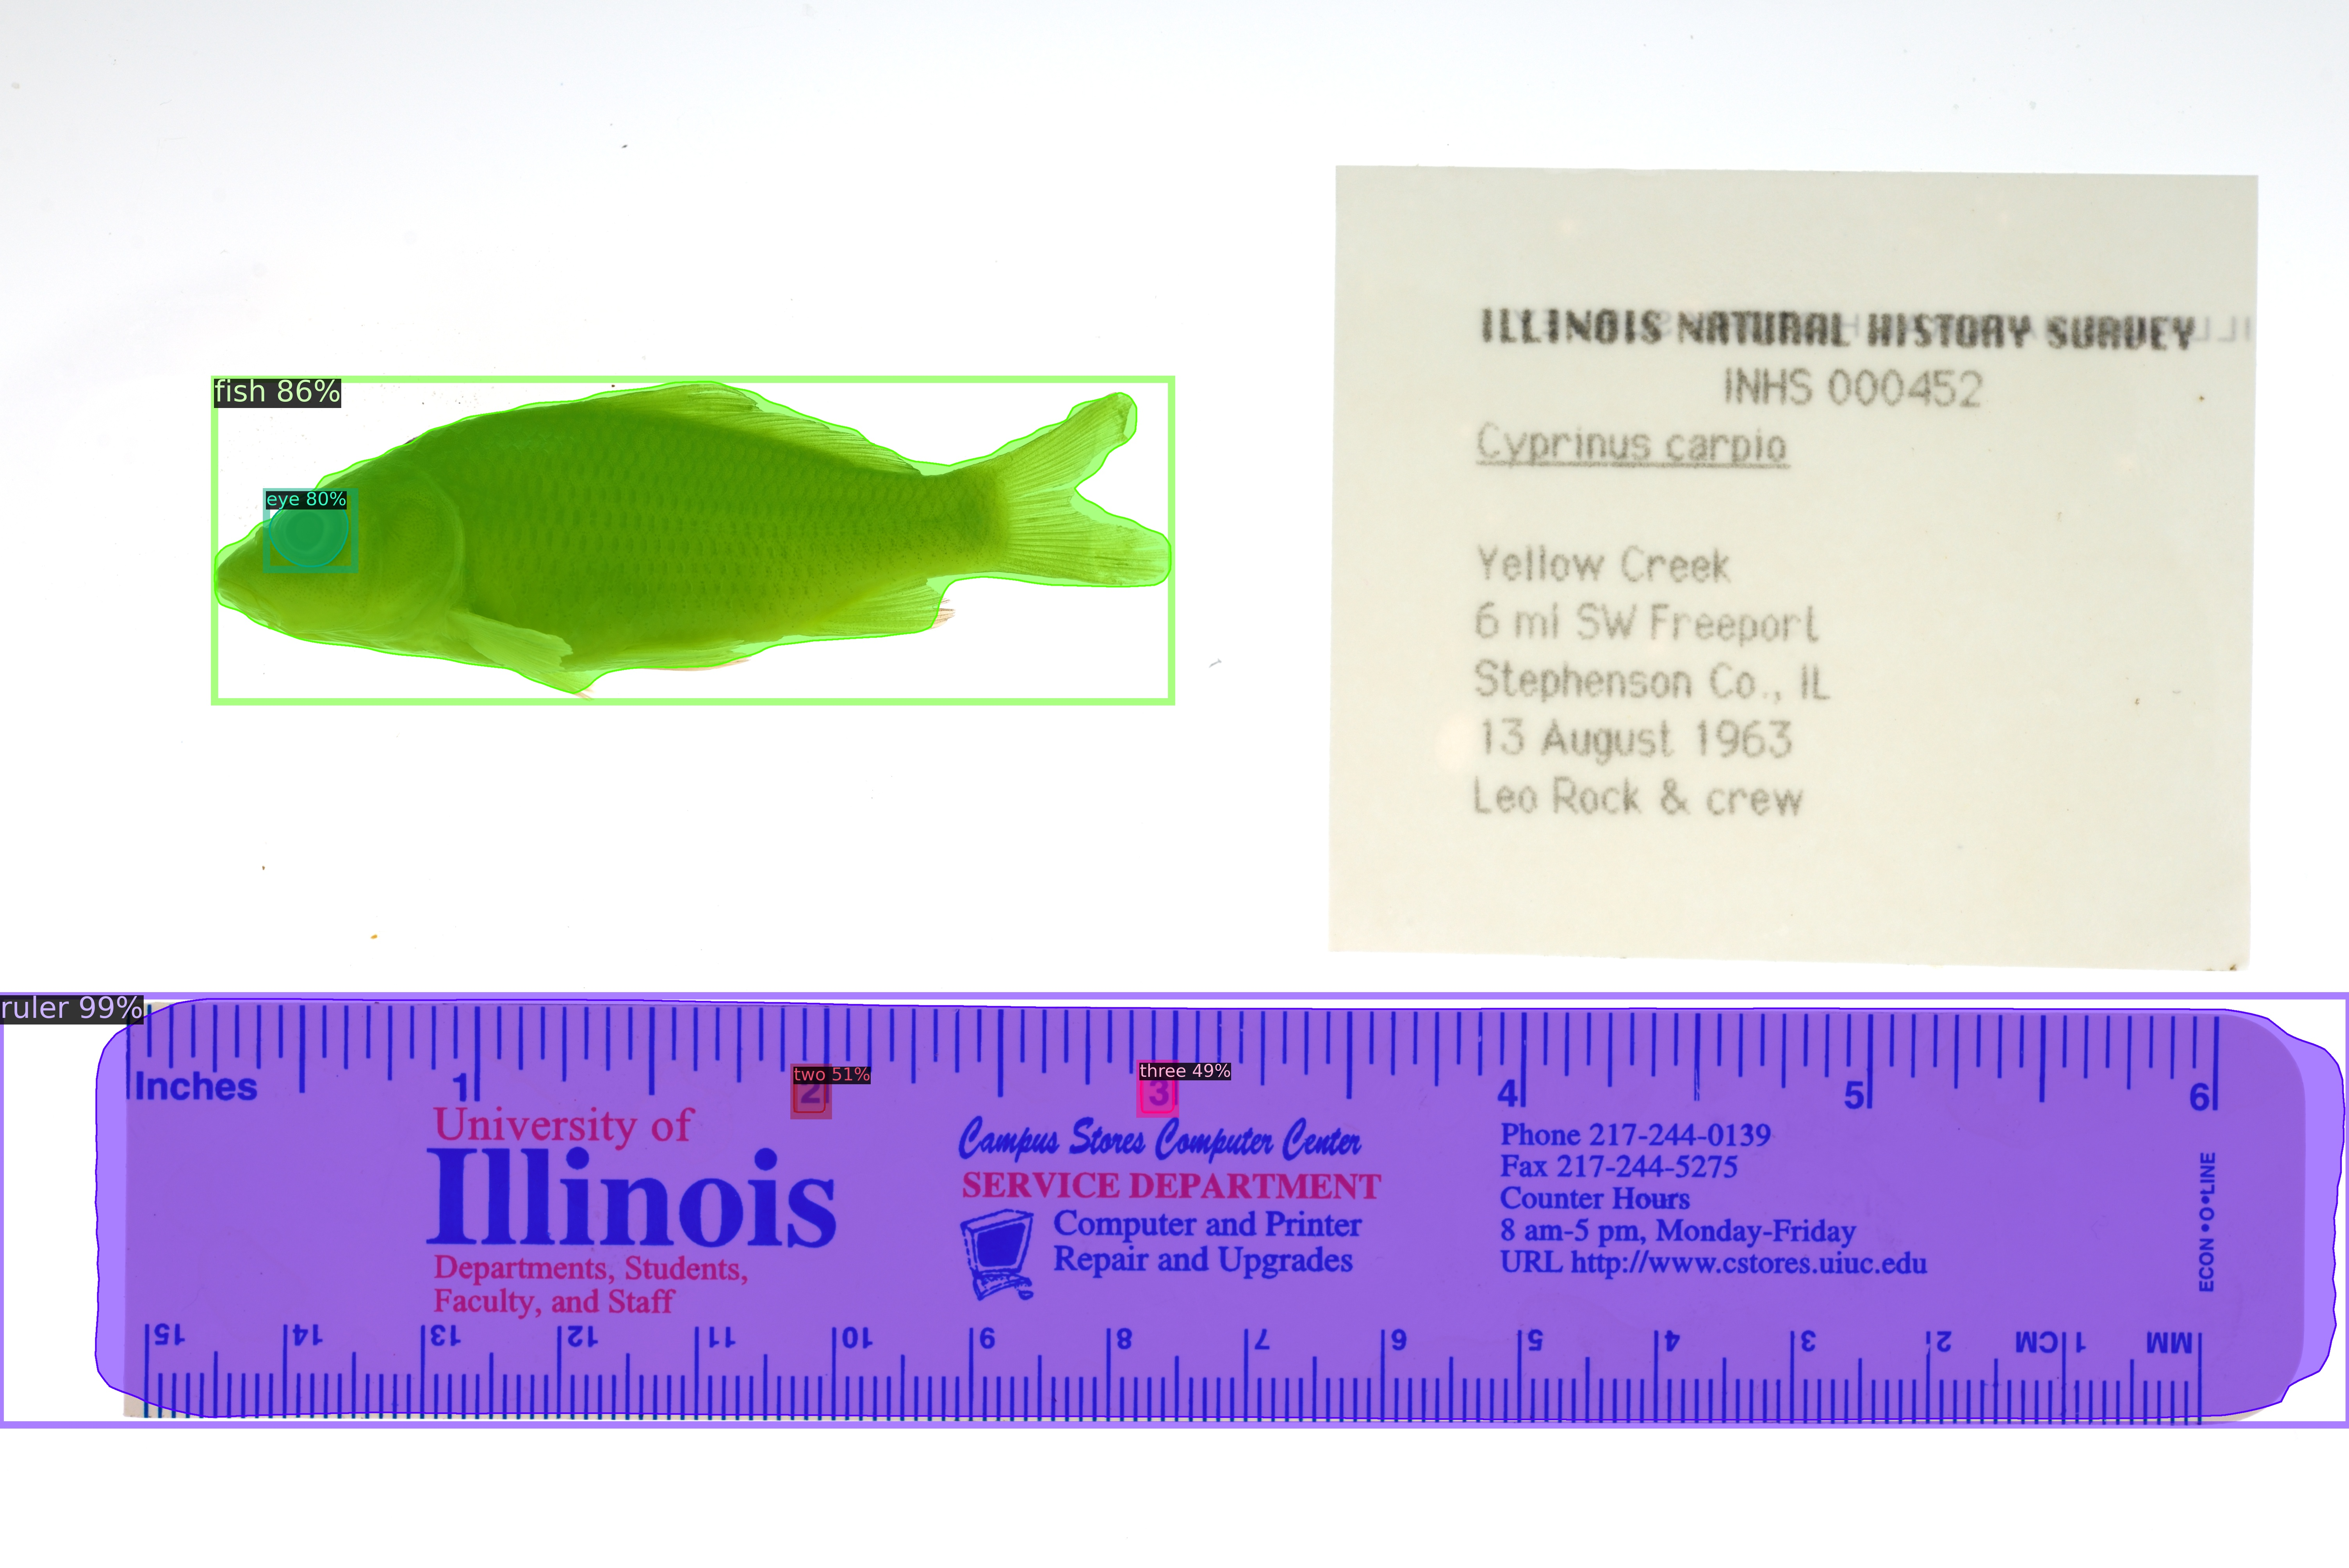
\includegraphics[width=\textwidth]{fish}
  \caption{Fish prediction}
  \Description{Fish prediction}
  \label{fig:fish}
\end{teaserfigure}

%%
%% This command processes the author and affiliation and title
%% information and builds the first part of the formatted document.
\maketitle

\section{Introduction}

\todo{Sentences I didn't use: Over the last few decades, cyberinfrastructure development, advances in digitization, and the open science tenor, have helped support global access to natural history. OR
Global access to natural history collections has accelerated over the last few decades to advances in cyberinfrastructure, digitization, and the general open science tenor}

Over the last several decades advances in computing, imaging, and cyberinfrastructure have supported the growth of digital natural history collection. In the U.S., programs, such as the National Science Foundation’s initial Advancing Digitization of Biodiversity Collections (ADBC) program, which ran for well over [nearly?] a decade, and the current Infrastructure Capacity for Biological Research program have supported the digital transformation of data and images for millions of biological specimens. These resources are globally available through a wide range of portals and digital libraries for researchers, educators, students, and the general public to examine and compare in ways previously unimaginable. Significant challenges surface; however, when researchers seek to apply computational methods, due to both image quality and metadata. (As researchers seek to apply computational methods, and explore AI, significant challenges surface..) 

Unfortunately, potential scientific advances are hindered [by image quality] as well as [more so?] the lack of high-quality and pertinent metadata associated with the image collections. Many specimen collections include Darwin Core metadata, detailing specimen taxon, geographic location, and several other descriptive aspects. Additionally, some digitization efforts record technical metadata, detailing imaging specifications. While these types of metadata are helpful for a human examining several images at a time, they are insufficient for researchers seeking to apply computational methods to examine thousands of images to determine if, for instance, a dorsal fin of a specific fish has a different shape. Since the collections may each contain tens of thousands of images, producing metadata for each image via a manual process is prohibitively labor-intensive and infeasible. Methods for automatically computing metadata from images are therefore needed to fully exploit biological image repositories for scientific discovery.~\cite{Leipzig2021.01.28.428644}\todo{Throwing in Jeremy's paper somewhere}

As a step towards improving metadata in specimen research image collections, members of the Metadata Research Center, Drexel University, have been developing methods to automatically analyze fish images and extract a set of important features [metadata]. The research is being conducted as part of Biology Guided Neural Networks (BGNN) project, which aims to develop a novel class of artificial neural networks that exploits machine readable and predictive knowledge associated with specimen images, phylogenies and anatomy ontologies. Using a combination of machine learning and image informatics tools and techniques, we can accurately determine general image quality and metadata such as fish quantity and location within images, fish orientation and other quantitative fish features, image scaling based on ruler identification and measurement. This paper reports on our research examining a set of [add numbers] images drawn from the Illinois Natural History Survey (INHS) Collection. The following section of this paper provides contextual background for this work, followed by the research goals and objectives, and a review of our research methods. Next, the results are presented, followed by a discussion. The conclusion highlights key findings and identifies next steps.

\section{Related Work}
Text~\todo[noline]{Do this}
\subsection{Metadata for Image Collection}
Metadata development is intertwined with the development of digital technology. A wide range of metadata standards are applicable to metadata supporting image description as well as technical aspects, and have been used in a range of image repositories. Examples of Descriptive schemes include X, y, z... Examples of technical schemes include... The use varies across communities, and application technique is primarily manual. Research evaluating such schemes XXX, show XXX. 

Natural history collections generally use a sub-set of such standards. Darwin Core, a globally adopted standard overseen by the Taxonomic Data Working Group (TDWG).  [Jane continue here on some of this, and then with preservation/image quality less]

\subsection{Metadata generation?}

\subsection{Fish Image Analysis}

\cite{BockAlexander2018TITE}
\cite{KonovalovD2017RDfA}
\cite{Williams:2020:UIF}

\section{Methods}
Our process for metadata generation can be broken into 3 steps: object detection with Facebook's Detectron2 machine learning library (subsequently referred to as \verb|detectron|), image informatics analysis at the pixel level, and calculations on the results of the previous steps to determine higher level metadata properties.

\subsection{Detectron}
A prerequisite task to addressing any more advanced metadata property determination is finding specimens (and other relevant objects) within collection images. Object detection has been an incredibly active field of study in recent years,~\cite{zou2019object} and has resulted in a number of well tested purpose built architectures. We elected to use Facebook AI Research's \verb|detectron| tool~\cite{wu2019detectron2}, and specifically its implementation of the Mask R-CNN architecture~\cite{he2018mask}, for object detection in our project.

\verb|detectron| is built on \verb|pytorch|~\cite{NEURIPS2019_9015} and provides a relatively straightforward method for training on COCO~\cite{DBLP:journals/corr/LinMBHPRDZ14} format dataset. It is able to handle an arbitrary number of object classes, and can classify an arbitrary number of object within a given sample. For our project, we are currently using it to identify five object classes: fish, fish eyes, rulers, and the numbers 2 and 3 on rulers.

Placeholder\todo{A paragraph about training will go here}
\subsection{Pixel Analysis}
The masks and bounding boxes produced by \verb|detectron| are generally quite good, although they are almost never perfect. They almost always either include additional background as part of the fish, or clip part(s) of the fish outside the bounding box. To solve this shortcoming, we utilize pixel analysis methods commonly found in image informatics.

The first calculation in the pixel analysis process is determining the cutoff intensity between what constitutes the foreground (i.e.\ the fish) and background of the image. Initially, we base this off the bounding box and mask generated by \verb|detectron|. Specimen images are read in as gray scale, and pixels in the image are treated as unsigned integers between 0 and 255. Otsu thresholding is used to get an initial cutoff value between foreground and background. \todo{Put in another sentence or two about Otsu} While this value occasionally generates an accurate mask as is, most of the time the contrast between foreground and background is not great enough and much of the lighter parts of the fish (such as its tail fin) are marked as background.

To overcome this, the threshold value needs either scaled up or down depending on if the background is lighter or darker than the fish. For our current dataset, the background is always lighter (i.e.\ closer to 255), so the threshold value needs scaled up to include more of the image as foreground. Precisely how much to scale this value by is difficult to determine. For optimal results it is dependent on the level of contrast between the background and foreground, which can be affected by both how washed out the image is and how light or dark the pigmentation of the fish is. To take this into account, we measure the mean intensity of the foreground and background, then use these intensity values and the difference between them to scale the threshold value. Even with these values in hand it is not entirely clear how to scale the threshold, but we have found\ldots{}\todo{This is still somewhat indeterminate, need to pick a definitive technique, I've tried a few}

While thresholding has the potential to generate better masks than a neural network (when provided an initial approximate bounding box), it also introduces considerable noise. Single or small groups of errant pixels can be marked as foreground depending on the consistency of the background, and interior pixels of the fish (especially around the fins) can be marked as background. To be useful for generating an accurate bounding box and for subsequent computational analysis, the mask must consist of one single ``blob'' over the fish the contains no holes, and no other pixels disconnected from this blob can be marked as foreground.

To accomplish this, we apply an iterative process of flood filling from all the foreground pixels in the image until a blob is generated that is large enough to constitute the fish. This is another metaparameter, but greater than 10\% of the current bounding box has masked the specimen in all observed cases. Once the fish's blob is found, noise then needs removed. This is done by flood filling from each of the corner of the bounding box where the specimen is not present (all four corners in the overwhelming majority of cases), then taking the inverse of the result. The fish mask is excluded from these corner flood fills, so this process removes all noise from both the background and foreground of the image leaving only a close mask over the fish itself.

With an accurate mask generated, it is then necessary to check whether the bounding box needs expanded or shrunk along any edges. Expansion is done first, buy checking whether any edge intersects with any of the foreground mask pixels. If one does, it is expanded out by 1 pixel. If any edges are expanded, the whole the process, masking and expansion process is repeated to account for any changes in average intensities. Once no edges contain foreground pixels, the mask is the shrunk. This process is more efficient as all that is required is to shrink each edge by one up until the point they contain one or more foreground pixels. Once the shrinkage step is accomplished, the final mask and bounding box have been generated.
\subsection{Metadata Generation}
Including what has already been discussed, the following metadata properties are being currently being generated:

\begin{table}[H]
    \centering
    \caption{Metadata properties}
    \label{tab:properties}
    \begin{tabular}{cccp{0.5\linewidth}}
        \toprule
        \textbf{Property} & \textbf{Association} & \textbf{Type} & \textbf{Explanation}\\
        \midrule
        \verb|has_fish| & Overall Image & Boolean & Whether a fish was found in the image.\\
        \verb|fish_count| & Overall Image & Integer & The quantity of fish present.\\
        \verb|has_ruler| & Overall Image & Boolean & Whether a ruler was found in the image.\\
        \verb|ruler_bbox| & Overall Image & 4 Tuple & The bounding box of the ruler (if found).\\
        \verb|scale| & Overall Image & Float & The scale of the image in \(\frac{\mathrm{pixels}}{\mathrm{cm}}\).\\
        \verb|bbox| & Per Fish & 4 Tuple & The top left and bottom right coordinates of what define the bounding box for a fish.\\
        \verb|background.mean| & Per Fish & Float & The mean intensity of the background within a given fish's bounding box.\\
        \verb|background.std| & Per Fish & Float & The standard deviation of the background within a given fish's bounding box.\\
        \verb|foreground.mean| & Per Fish & Float & The mean intensity of the foreground within a given fish's bounding box.\\
        \verb|foreground.std| & Per Fish & Float & The standard deviation of the foreground within a given fish's bounding box.\\
        \verb|centroid| & Per Fish & 4 Tuple & The centroid of a given fish's bitmask.\\
        \verb|primary_axis| & Per Fish & 2D Vector & The unit length primary axis (eigenvector) for the bitmask of a given fish.\\
        \verb|clock_value| & Per Fish & Integer & A fish's primary axis converted into an integer ``clock value'' between 1 and 12.\\
        \verb|length| & Per Fish & Float & The length of a fish in \(\frac{\mathrm{pixels}}{\mathrm{cm}}\).\\
        \verb|mask| & Per Fish & 2D Matrix & The bitmask of a fish in 0's and 1's.\\
        \verb|score| & Per Fish & Float & The percent confidence score output by \verb|detectron| for a given fish.\\
        \verb|has_eye| & Per Fish & Boolean & Whether an eye was found for a given fish.\\
        \verb|eye_center| & Per Fish & 2 Tuple & The centroid of a fish's eye.\\
        \verb|side| & Per Fish & String & The side (i.e.\ \verb|'left'| or \verb|'right'|) of the fish that is facing the camera (dependent on finding its eye).\\
      \bottomrule
\end{tabular}
\end{table}

\verb|has_fish|, \verb|fish_count|, \verb|has_ruler|, \verb|ruler_bbox|, \verb|background.*|, \verb|foreground.*|, \verb|bbox|, \verb|mask|, \verb|score|, and \verb|has_eye| have already been discussed. The remaining properties are determined as follows:
\subsubsection{centroid and eye\_center}
Centroids are provided for masks/bounding boxes generated by \verb|detectron|, and since we do not recalculate the mask of fish eyes we can use that value directly for \verb|eye_center|.

Since we recalculate the mask of the fish, we must recalculate its centroid as well. This can be done via
\begin{equation}
    (\bar{x}, \bar{y}) = (\mathrm{round}(\frac{M_{10}}{M_{00}}), \mathrm{round}(\frac{M_{01}}{M_{00}}))
\end{equation}
where \(M_{00}\) is the pixel area of the fish's blob, \(M_{10}\) is the sum of all the \(x\) values of blob pixels, and \(M_{01}\) is the sum of all the \(y\) values of blob pixels.
\subsubsection{side}
Determining which \verb|side| of the fish is visible is predicated on finding its eye. If an eye is found, the sign of the \(x\) component of the vector from the centroid of the fish to the centroid of the eye specifies which side is up: negative for left and positive for right. This assumes the fish was photographed vertically, which is essentially always the case for all image collections our group has worked on.
\subsubsection{primary\_axis and clock\_value}
The \verb|primary_axis| of a fish can be calculated by taking the covariance\todo{I could explain this in more detail if necessary} of its blob in \(x\) and \(y\), which yields its principle eigenvector. This can be directly assigned to the property. If an eye is present, we specify this axis in the direction of the eye in relation to the fish's centroid.

Our team encoded this information as a ``clock value'' between 1 and 12 when recording it by hand. To convert \verb|principal_axis| to \verb|clock_value|, the sign of \(x\) and \(y\) on the principal axis are used to determine which Cartesian quadrant the fish is angles into relative to its centroid. Depending on this quadrant, we then dot product the principal axis with either \([-1,0]\), \([0,-1]\), \([1,0]\) or \([0,1]\) which correspond to 9, 6, 3 and ``0'' o'clock respectively. The resulting radian value is then converted to a polar displacement in clock value space, and added to the comparative clock value used in the dot product. This then gives the fish's clock value from 0 to \(11.\overline{9}\). Before recording as \verb|clock_value| in the output, the value is rounded to the nearest integer, and in the event of a 0 final result it is replaced with 12.
\subsubsection{scale and length}
\(\frac{\mathrm{pixels}}{\mathrm{inch}}\) can be calculated by measuring the distance between the digits 2 and 3 found on the ruler by \verb|detectron|. Converting this to \(\frac{\mathrm{pixels}}{\mathrm{cm}}\) gives the \verb|scale| metadata property as reported in the output.

For the fish \verb|length| property, it is necessary to determine the furthest points from the centroid of the fish in each direction. Since fish are normally measured in a straight line from their snout down the middle of their trunk, we project every pixel onto the major axis of the fish (as a line through its centroid) before checking the distance. This projection is done by intersecting the line through the point along the tangent of the principal axis and the aforementioned centroid--principal axis line. After checking every pixel, measuring the distance between the two furthest projected points gives the length of the fish in pixels. Multiplying this by \verb|scale| gives the fish \verb|length| in centimeters.
\subsection{Consideration}
Just gonna throw some caveats in here, might be its own section might not
\begin{itemize}
    \item Program falls back to using detectron mask and bbox for metadata generation in the event the mask generation/pixel analysis fails. Failure is defined as never finding a cohesive flood filled mask that covers more than 10\% of the detectron bbox initially. Can provide a statistic on how often this occurs.
\end{itemize}
\section{Results}
\begin{verbatim}
What I think should be the final results:

Right: 6956
Errored: 0
No eye: 246
No fish: 10
Wrong wrong: 35
Total: 7247
Percent right: 0.959845453291017
Percent right that didn't error: 0.9949935631526248

-----------------------

My hand checking of the ''wrong wrong'' fish:

INHS_FISH_101109.jpg: 9, 11, I'm wrong although it's fairly curved
INHS_FISH_56818.jpg: 4, 2, I'm wrong although there's a tag that is likely messing things up
INHS_FISH_57607.jpg: 3, 9, I'm wrong
INHS_FISH_57001.jpg: 4, 2, I'm wrong although there's a tag that is likely messing things up
INHS_FISH_63953.jpg: 3, 9, I'm wrong
INHS_FISH_51100.jpg: 3, 9, I'm wrong
INHS_FISH_80528.jpg: 3, 8, I'm wrong
INHS_FISH_6370.jpg: 3, 9, I'm wrong
INHS_FISH_54157.jpg: 9, 7, I'm arguably wrong although it's very curved
INHS_FISH_80987.jpg: 9, 3, I'm wrong although this one is a fairly atypical image

INHS_FISH_58647.jpg: 9, 7, I'm right
INHS_FISH_8415.jpg: 9, 6, I'm right
INHS_FISH_5041.jpg: 9, 11, very curved averages to about 9
INHS_FISH_52821.jpg: 9, 7, I'm arguably right although the fish is damaged and its head points to ~7
INHS_FISH_6696.jpg: 9, 7, I'm right
INHS_FISH_75252.jpg: 9, 6, I'm right
INHS_FISH_79498.jpg: 9, 6, I'm right
INHS_FISH_45744.jpg: 9, 5, I'm right
INHS_FISH_47579.jpg: 9, 6, I'm right
INHS_FISH_64599.jpg: 9, 6, I'm right
INHS_FISH_74550.jpg: 9, 5, I'm right
INHS_FISH_101664.jpg: 9, 6, I'm right
INHS_FISH_100861.jpg: 9, 6, I'm right
INHS_FISH_60589.jpg: 3, 9, I'm right
INHS_FISH_53469.jpg: 9, 1, I'm right
INHS_FISH_44694.jpg: 9, 6, I'm right
INHS_FISH_54921.jpg: 9, 6, I'm right
INHS_FISH_44645.jpg: 10, 8, I'm right
INHS_FISH_50459.jpg: 9, 11, I'm right although the fish is damaged and its head points to ~11
INHS_FISH_68061.jpg: 9, 6, I'm right
INHS_FISH_74716.jpg: 9, 6, I'm right
INHS_FISH_80976.jpg: 9, 6, I'm right
INHS_FISH_57977.jpg: 9, 6, I'm right
INHS_FISH_45377.jpg: 9, 6, I'm right
INHS_FISH_47142.jpg: 9, 6, I'm right

Verdict: For only 10 of the 35 am I actually wrong and all of those are either curved, atypical
images with tags, or something on the wrong side was detected as an eye (so the clock value is backwards).

\end{verbatim}
\section{Discussion}
Text \textit{texty text}%~\cite{Lamport:LaTeX}
\section{Conclusion}
Text \textbf{text}

\bibliographystyle{ACM-Reference-Format}
\bibliography{paper}

\begin{comment}
\pagebreak{}
\section{Introduction}~\label{demo-intro}
ACM's consolidated article template, introduced in 2017, provides a
consistent \LaTeX\ style for use across ACM publications, and
incorporates accessibility and metadata-extraction functionality
necessary for future Digital Library endeavors. Numerous ACM and
SIG-specific \LaTeX\ templates have been examined, and their unique
features incorporated into this single new template.

If you are new to publishing with ACM, this document is a valuable
guide to the process of preparing your work for publication. If you
have published with ACM before, this document provides insight and
instruction into more recent changes to the article template.

The ``\verb|acmart|'' document class can be used to prepare articles
for any ACM publication --- conference or journal, and for any stage
of publication, from review to final ``camera-ready'' copy, to the
author's own version, with {\itshape very} few changes to the source.

\section{Template Overview}
As noted in the introduction, the ``\verb|acmart|'' document class can
be used to prepare many different kinds of documentation --- a
double-blind initial submission of a full-length technical paper, a
two-page SIGGRAPH Emerging Technologies abstract, a ``camera-ready''
journal article, a SIGCHI Extended Abstract, and more --- all by
selecting the appropriate {\itshape template style} and {\itshape
  template parameters}.

This document will explain the major features of the document
class. For further information, the {\itshape \LaTeX\ User's Guide} is
available from
\url{https://www.acm.org/publications/proceedings-template}.

\subsection{Template Styles}

The primary parameter given to the ``\verb|acmart|'' document class is
the {\itshape template style} which corresponds to the kind of publication
or SIG publishing the work. This parameter is enclosed in square
brackets and is a part of the {\verb|documentclass|} command:
\begin{verbatim}
  \documentclass[STYLE]{acmart}
\end{verbatim}

Journals use one of three template styles. All but three ACM journals
use the {\verb|acmsmall|} template style:
\begin{itemize}
\item {\verb|acmsmall|}: The default journal template style.
\item {\verb|acmlarge|}: Used by JOCCH and TAP.
\item {\verb|acmtog|}: Used by TOG.
\end{itemize}

The majority of conference proceedings documentation will use the {\verb|acmconf|} template style.
\begin{itemize}
\item {\verb|acmconf|}: The default proceedings template style.
\item{\verb|sigchi|}: Used for SIGCHI conference articles.
\item{\verb|sigchi-a|}: Used for SIGCHI ``Extended Abstract'' articles.
\item{\verb|sigplan|}: Used for SIGPLAN conference articles.
\end{itemize}

\subsection{Template Parameters}

In addition to specifying the {\itshape template style} to be used in
formatting your work, there are a number of {\itshape template parameters}
which modify some part of the applied template style. A complete list
of these parameters can be found in the {\itshape \LaTeX\ User's Guide.}

Frequently-used parameters, or combinations of parameters, include:
\begin{itemize}
\item {\verb|anonymous,review|}: Suitable for a ``double-blind''
  conference submission. Anonymizes the work and includes line
  numbers. Use with the \verb|\acmSubmissionID| command to print the
  submission's unique ID on each page of the work.
\item{\verb|authorversion|}: Produces a version of the work suitable
  for posting by the author.
\item{\verb|screen|}: Produces colored hyperlinks.
\end{itemize}

This document uses the following string as the first command in the
source file:
\begin{verbatim}
\documentclass[acmsmall]{acmart}
\end{verbatim}

\section{Modifications}

Modifying the template --- including but not limited to: adjusting
margins, typeface sizes, line spacing, paragraph and list definitions,
and the use of the \verb|\vspace| command to manually adjust the
vertical spacing between elements of your work --- is not allowed.

{\bfseries Your document will be returned to you for revision if
  modifications are discovered.}

\section{Typefaces}

The ``\verb|acmart|'' document class requires the use of the
``Libertine'' typeface family. Your \TeX\ installation should include
this set of packages. Please do not substitute other typefaces. The
``\verb|lmodern|'' and ``\verb|ltimes|'' packages should not be used,
as they will override the built-in typeface families.

\section{Title Information}

The title of your work should use capital letters appropriately -
\url{https://capitalizemytitle.com/} has useful rules for
capitalization. Use the {\verb|title|} command to define the title of
your work. If your work has a subtitle, define it with the
{\verb|subtitle|} command.  Do not insert line breaks in your title.

If your title is lengthy, you must define a short version to be used
in the page headers, to prevent overlapping text. The \verb|title|
command has a ``short title'' parameter:
\begin{verbatim}
  \title[short title]{full title}
\end{verbatim}

\section{Authors and Affiliations}

Each author must be defined separately for accurate metadata
identification. Multiple authors may share one affiliation. Authors'
names should not be abbreviated; use full first names wherever
possible. Include authors' e-mail addresses whenever possible.

Grouping authors' names or e-mail addresses, or providing an ``e-mail
alias,'' as shown below, is not acceptable:
\begin{verbatim}
  \author{Brooke Aster, David Mehldau}
  \email{dave,judy,steve@university.edu}
  \email{firstname.lastname@phillips.org}
\end{verbatim}

The \verb|authornote| and \verb|authornotemark| commands allow a note
to apply to multiple authors --- for example, if the first two authors
of an article contributed equally to the work.

If your author list is lengthy, you must define a shortened version of
the list of authors to be used in the page headers, to prevent
overlapping text. The following command should be placed just after
the last \verb|\author{}| definition:
\begin{verbatim}
  \renewcommand{\shortauthors}{McCartney, et al.}
\end{verbatim}
Omitting this command will force the use of a concatenated list of all
of the authors' names, which may result in overlapping text in the
page headers.

The article template's documentation, available at
\url{https://www.acm.org/publications/proceedings-template}, has a
complete explanation of these commands and tips for their effective
use.

Note that authors' addresses are mandatory for journal articles.

\section{Rights Information}

Authors of any work published by ACM will need to complete a rights
form. Depending on the kind of work, and the rights management choice
made by the author, this may be copyright transfer, permission,
license, or an OA (open access) agreement.

Regardless of the rights management choice, the author will receive a
copy of the completed rights form once it has been submitted. This
form contains \LaTeX\ commands that must be copied into the source
document. When the document source is compiled, these commands and
their parameters add formatted text to several areas of the final
document:
\begin{itemize}
\item the ``ACM Reference Format'' text on the first page.
\item the ``rights management'' text on the first page.
\item the conference information in the page header(s).
\end{itemize}

Rights information is unique to the work; if you are preparing several
works for an event, make sure to use the correct set of commands with
each of the works.

The ACM Reference Format text is required for all articles over one
page in length, and is optional for one-page articles (abstracts).

\section{CCS Concepts and User-Defined Keywords}

Two elements of the ``acmart'' document class provide powerful
taxonomic tools for you to help readers find your work in an online
search.

The ACM Computing Classification System ---
\url{https://www.acm.org/publications/class-2012} --- is a set of
classifiers and concepts that describe the computing
discipline. Authors can select entries from this classification
system, via \url{https://dl.acm.org/ccs/ccs.cfm}, and generate the
commands to be included in the \LaTeX\ source.

User-defined keywords are a comma-separated list of words and phrases
of the authors' choosing, providing a more flexible way of describing
the research being presented.

CCS concepts and user-defined keywords are required for for all
articles over two pages in length, and are optional for one- and
two-page articles (or abstracts).

\section{Sectioning Commands}

Your work should use standard \LaTeX\ sectioning commands:
\verb|section|, \verb|subsection|, \verb|subsubsection|, and
\verb|paragraph|. They should be numbered; do not remove the numbering
from the commands.

Simulating a sectioning command by setting the first word or words of
a paragraph in boldface or italicized text is {\bfseries not allowed.}

\section{Tables}

The ``\verb|acmart|'' document class includes the ``\verb|booktabs|''
package --- \url{https://ctan.org/pkg/booktabs} --- for preparing
high-quality tables.

Table captions are placed {\itshape above} the table.

Because tables cannot be split across pages, the best placement for
them is typically the top of the page nearest their initial cite.  To
ensure this proper ``floating'' placement of tables, use the
environment \textbf{table} to enclose the table's contents and the
table caption.  The contents of the table itself must go in the
\textbf{tabular} environment, to be aligned properly in rows and
columns, with the desired horizontal and vertical rules.  Again,
detailed instructions on \textbf{tabular} material are found in the
\textit{\LaTeX\ User's Guide}.

Immediately following this sentence is the point at which
Table~\ref{tab:freq} is included in the input file; compare the
placement of the table here with the table in the printed output of
this document.

\begin{table}
  \caption{Frequency of Special Characters}
  \label{tab:freq}
  \begin{tabular}{ccl}
    \toprule
    Non-English or Math&Frequency&Comments\\
    \midrule
    \O & 1 in 1,000& For Swedish names\\
    $\pi$ & 1 in 5& Common in math\\
    \$ & 4 in 5 & Used in business\\
    $\Psi^2_1$ & 1 in 40,000& Unexplained usage\\
  \bottomrule
\end{tabular}
\end{table}

To set a wider table, which takes up the whole width of the page's
live area, use the environment \textbf{table*} to enclose the table's
contents and the table caption.  As with a single-column table, this
wide table will ``float'' to a location deemed more
desirable. Immediately following this sentence is the point at which
Table~\ref{tab:commands} is included in the input file; again, it is
instructive to compare the placement of the table here with the table
in the printed output of this document.

\begin{table*}
  \caption{Some Typical Commands}
  \label{tab:commands}
  \begin{tabular}{ccl}
    \toprule
    Command &A Number & Comments\\
    \midrule
    \texttt{{\char'134}author} & 100& Author \\
    \texttt{{\char'134}table}& 300 & For tables\\
    \texttt{{\char'134}table*}& 400& For wider tables\\
    \bottomrule
  \end{tabular}
\end{table*}

Always use midrule to separate table header rows from data rows, and
use it only for this purpose. This enables assistive technologies to
recognise table headers and support their users in navigating tables
more easily.

\section{Math Equations}
You may want to display math equations in three distinct styles:
inline, numbered or non-numbered display.  Each of the three are
discussed in the next sections.

\subsection{Inline (In-text) Equations}
A formula that appears in the running text is called an inline or
in-text formula.  It is produced by the \textbf{math} environment,
which can be invoked with the usual
\texttt{{\char'134}begin\,\ldots{\char'134}end} construction or with
the short form \texttt{\$\,\ldots\$}. You can use any of the symbols
and structures, from $\alpha$ to $\omega$, available in
\LaTeX~\cite{Lamport:LaTeX}; this section will simply show a few
examples of in-text equations in context. Notice how this equation:
\begin{math}
  \lim_{n\rightarrow \infty}x=0
\end{math},
set here in in-line math style, looks slightly different when
set in display style.  (See next section).

\subsection{Display Equations}
A numbered display equation---one set off by vertical space from the
text and centered horizontally---is produced by the \textbf{equation}
environment. An unnumbered display equation is produced by the
\textbf{displaymath} environment.

Again, in either environment, you can use any of the symbols and
structures available in \LaTeX\@; this section will just give a couple
of examples of display equations in context.  First, consider the
equation, shown as an inline equation above:
\begin{equation}
  \lim_{n\rightarrow \infty}x=0
\end{equation}
Notice how it is formatted somewhat differently in
the \textbf{displaymath}
environment.  Now, we'll enter an unnumbered equation:
\begin{displaymath}
  \sum_{i=0}^{\infty} x + 1
\end{displaymath}
and follow it with another numbered equation:
\begin{equation}
  \sum_{i=0}^{\infty}x_i=\int_{0}^{\pi+2} f
\end{equation}
just to demonstrate \LaTeX's able handling of numbering.

\section{Figures}

The ``\verb|figure|'' environment should be used for figures. One or
more images can be placed within a figure. If your figure contains
third-party material, you must clearly identify it as such, as shown
in the example below.
\begin{figure}[h]
  \centering
  %\includegraphics[width=\linewidth]{sample-franklin}
  \caption{1907 Franklin Model D roadster. Photograph by Harris \&
    Ewing, Inc. [Public domain], via Wikimedia
    Commons. (\url{https://goo.gl/VLCRBB}).}
  \Description{A woman and a girl in white dresses sit in an open car.}
\end{figure}

Your figures should contain a caption which describes the figure to
the reader.

Figure captions are placed {\itshape below} the figure.

Every figure should also have a figure description unless it is purely
decorative. These descriptions convey what’s in the image to someone
who cannot see it. They are also used by search engine crawlers for
indexing images, and when images cannot be loaded.

A figure description must be unformatted plain text less than 2000
characters long (including spaces).  {\bfseries Figure descriptions
  should not repeat the figure caption – their purpose is to capture
  important information that is not already provided in the caption or
  the main text of the paper.} For figures that convey important and
complex new information, a short text description may not be
adequate. More complex alternative descriptions can be placed in an
appendix and referenced in a short figure description. For example,
provide a data table capturing the information in a bar chart, or a
structured list representing a graph.  For additional information
regarding how best to write figure descriptions and why doing this is
so important, please see
\url{https://www.acm.org/publications/taps/describing-figures/}.

\subsection{The ``Teaser Figure''}

A ``teaser figure'' is an image, or set of images in one figure, that
are placed after all author and affiliation information, and before
the body of the article, spanning the page. If you wish to have such a
figure in your article, place the command immediately before the
\verb|\maketitle| command:
\begin{verbatim}
  \begin{teaserfigure}
    \includegraphics[width=\textwidth]{sampleteaser}
    \caption{figure caption}
    \Description{figure description}
  \end{teaserfigure}
\end{verbatim}

\section{Citations and Bibliographies}

The use of \BibTeX\ for the preparation and formatting of one's
references is strongly recommended. Authors' names should be complete
--- use full first names (``Donald E. Knuth'') not initials
(``D. E. Knuth'') --- and the salient identifying features of a
reference should be included: title, year, volume, number, pages,
article DOI, etc.

The bibliography is included in your source document with these two
commands, placed just before the \verb|\end{document}| command:
\begin{verbatim}
  \bibliographystyle{ACM-Reference-Format}
  \bibliography{bibfile}
\end{verbatim}
where ``\verb|bibfile|'' is the name, without the ``\verb|.bib|''
suffix, of the \BibTeX\ file.

Citations and references are numbered by default. A small number of
ACM publications have citations and references formatted in the
``author year'' style; for these exceptions, please include this
command in the {\bfseries preamble} (before the command
``\verb|\begin{document}|'') of your \LaTeX\ source:
\begin{verbatim}
  \citestyle{acmauthoryear}
\end{verbatim}

  Some examples.  A paginated journal article \cite{Abril07}, an
  enumerated journal article \cite{Cohen07}, a reference to an entire
  issue \cite{JCohen96}, a monograph (whole book) \cite{Kosiur01}, a
  monograph/whole book in a series (see 2a in spec. document)
  \cite{Harel79}, a divisible-book such as an anthology or compilation
  \cite{Editor00} followed by the same example, however we only output
  the series if the volume number is given \cite{Editor00a} (so
  Editor00a's series should NOT be present since it has no vol. no.),
  a chapter in a divisible book \cite{Spector90}, a chapter in a
  divisible book in a series \cite{Douglass98}, a multi-volume work as
  book \cite{Knuth97}, a couple of articles in a proceedings (of a
  conference, symposium, workshop for example) (paginated proceedings
  article) \cite{Andler79, Hagerup1993}, a proceedings article with
  all possible elements \cite{Smith10}, an example of an enumerated
  proceedings article \cite{VanGundy07}, an informally published work
  \cite{Harel78}, a couple of preprints \cite{Bornmann2019,
    AnzarootPBM14}, a doctoral dissertation \cite{Clarkson85}, a
  master's thesis: \cite{anisi03}, an online document / world wide web
  resource \cite{Thornburg01, Ablamowicz07, Poker06}, a video game
  (Case 1) \cite{Obama08} and (Case 2) \cite{Novak03} and \cite{Lee05}
  and (Case 3) a patent \cite{JoeScientist001}, work accepted for
  publication \cite{rous08}, 'YYYYb'-test for prolific author
  \cite{SaeediMEJ10} and \cite{SaeediJETC10}. Other cites might
  contain 'duplicate' DOI and URLs (some SIAM articles)
  \cite{Kirschmer:2010:AEI:1958016.1958018}. Boris / Barbara Beeton:
  multi-volume works as books \cite{MR781536} and \cite{MR781537}. A
  couple of citations with DOIs:
  \cite{2004:ITE:1009386.1010128,Kirschmer:2010:AEI:1958016.1958018}. Online
  citations: \cite{TUGInstmem, Thornburg01, CTANacmart}. Artifacts:
  \cite{R} and \cite{UMassCitations}.

\section{Acknowledgments}

Identification of funding sources and other support, and thanks to
individuals and groups that assisted in the research and the
preparation of the work should be included in an acknowledgment
section, which is placed just before the reference section in your
document.

This section has a special environment:
\begin{verbatim}
  \begin{acks}
  ...
  \end{acks}
\end{verbatim}
so that the information contained therein can be more easily collected
during the article metadata extraction phase, and to ensure
consistency in the spelling of the section heading.

Authors should not prepare this section as a numbered or unnumbered {\verb|\section|}; please use the ``{\verb|acks|}'' environment.

\section{Appendices}

If your work needs an appendix, add it before the
``\verb|\end{document}|'' command at the conclusion of your source
document.

Start the appendix with the ``\verb|appendix|'' command:
\begin{verbatim}
  \appendix
\end{verbatim}
and note that in the appendix, sections are lettered, not
numbered. This document has two appendices, demonstrating the section
and subsection identification method.

\section{SIGCHI Extended Abstracts}

The ``\verb|sigchi-a|'' template style (available only in \LaTeX\ and
not in Word) produces a landscape-orientation formatted article, with
a wide left margin. Three environments are available for use with the
``\verb|sigchi-a|'' template style, and produce formatted output in
the margin:
\begin{itemize}
\item {\verb|sidebar|}:  Place formatted text in the margin.
\item {\verb|marginfigure|}: Place a figure in the margin.
\item {\verb|margintable|}: Place a table in the margin.
\end{itemize}

%%
%% The acknowledgments section is defined using the "acks" environment
%% (and NOT an unnumbered section). This ensures the proper
%% identification of the section in the article metadata, and the
%% consistent spelling of the heading.
\begin{acks}
To Robert, for the bagels and explaining CMYK and color spaces.
\end{acks}

%%
%% The next two lines define the bibliography style to be used, and
%% the bibliography file.

\bibliographystyle{ACM-Reference-Format}
\bibliography{paper}

%%
%% If your work has an appendix, this is the place to put it.
\appendix

\section{Research Methods}

\subsection{Part One}

Lorem ipsum dolor sit amet, consectetur adipiscing elit. Morbi
malesuada, quam in pulvinar varius, metus nunc fermentum urna, id
sollicitudin purus odio sit amet enim. Aliquam ullamcorper eu ipsum
vel mollis. Curabitur quis dictum nisl. Phasellus vel semper risus, et
lacinia dolor. Integer ultricies commodo sem nec semper.

\subsection{Part Two}

Etiam commodo feugiat nisl pulvinar pellentesque. Etiam auctor sodales
ligula, non varius nibh pulvinar semper. Suspendisse nec lectus non
ipsum convallis congue hendrerit vitae sapien. Donec at laoreet
eros. Vivamus non purus placerat, scelerisque diam eu, cursus
ante. Etiam aliquam tortor auctor efficitur mattis.

\section{Online Resources}

Nam id fermentum dui. Suspendisse sagittis tortor a nulla mollis, in
pulvinar ex pretium. Sed interdum orci quis metus euismod, et sagittis
enim maximus. Vestibulum gravida massa ut felis suscipit
congue. Quisque mattis elit a risus ultrices commodo venenatis eget
dui. Etiam sagittis eleifend elementum.

Nam interdum magna at lectus dignissim, ac dignissim lorem
rhoncus. Maecenas eu arcu ac neque placerat aliquam. Nunc pulvinar
massa et mattis lacinia.

\end{comment}

\end{document}
\endinput
%%
%% End of file `sample-acmsmall-conf.tex'.
